\documentclass{article}
\usepackage[a4paper,top=2cm,bottom=2cm,left=2cm,right=2cm]{geometry}
\usepackage{graphicx} % Required for inserting images
\usepackage{algorithm}
\usepackage{algpseudocode}
\usepackage{algorithmicx}
\usepackage{amsmath}
\usepackage{tcolorbox}
\tcbuselibrary{listings, breakable}

\title{Bitonic Sort with CUDA}
\author{Georgios Rousomanis (10703) \\ 
Aistotle University of Thessaloniki \\ 
Department of Electrical and Computer engineering \\
email: }
\date{August 2025}

% Section and subsection numbering style
\renewcommand{\thesection}{V\arabic{section}}
\renewcommand{\thesubsection}{\arabic{section}.\arabic{subsection}}
\setcounter{section}{-1}
\setcounter{subsection}{-1}

\begin{document}

\maketitle

\section*{Introduction}

\section{Naive Global-Memory Bitonic Sort}

This version represents the most basic GPU implementation of the Bitonic Sort algorithm. The key goal of this 
version is correctness and a functional mapping of the bitonic sorting network onto the GPU. Each 
compare-and-swap operation in the sorting network is implemented as a separate kernel launch. All data resides 
in global memory, and no attempt is made to share or reuse data between threads. While simple and easy to debug, 
this approach is inefficient due to frequent kernel invocations and the lack of memory locality. This version 
serves as the baseline for evaluating future optimizations.

The GPU kernel performs the basic compare-and-swap step of the bitonic sorting network. Each thread operates on 
single index and computes its partner $j$ using the bitonic sort logic ($j = i \oplus step$). Only one of the two 
indices (the smaller one) performs the swap to avoid duplicate work. The direction of the comparison (ascending or
descending) depends on the current size of the bitonic sequence and the index of the thread.

\begin{algorithm}[H]
\caption{Compare-And-Swap Kernel (v0)}
\begin{algorithmic}[1]
\Procedure{CompareAndSwapKernelV0}{$data$, $n$, $size$, $step$}
    \State $i \gets$ global thread index
    \If{$i \geq n$} \Return \EndIf
    \State $j \gets i \oplus step$
    \If{$j > i$}
        \State $ascending \gets (i \ \&\ size) == 0$
        \State \Call{CompareAndSwap}{$data$, $i$, $j$, $ascending$}
    \EndIf
\EndProcedure
\end{algorithmic}
\end{algorithm}

The host code runs two nested loops: the outer loop iterates over the sizes of the bitonic sequences, and the 
inner loop performs the necessary merge steps by repeatedly launching the device kernel. Reversing at the end 
allows the core logic to always sort in ascending order, simplifying the kernel logic. Because every operation 
interacts with global memory, performance is limited -- especially due to the overhead of many kernel launches 
and the lack of shared memory usage.

\begin{algorithm}[H]
\caption{Bitonic Sort Driver (v0)}
\begin{algorithmic}[1]
\Procedure{BitonicSortV0}{$host\_data$, $n$, $descending$}
    \State Allocate $device\_data$ on GPU
    \State Copy $host\_data$ to $device\_data$
    
    \For{$size = 2$ to $n$ by $\times 2$}
        \For{$step = size / 2$ down to $1$ by $\div 2$}
            \State Launch \Call{CompareAndSwapKernelV0}{$device\_data$, $n$, $size$, $step$}
            \State Synchronize and check for errors
        \EndFor
    \EndFor

    \If{$descending$}
        \State Launch \Call{ReverseKernel}{$device\_data$, $n$}
        \State Synchronize and check for errors
    \EndIf

    \State Copy $device\_data$ back to $host\_data$
    \State Free GPU memory
\EndProcedure
\end{algorithmic}
\end{algorithm}


%%%%%%%%%%%%%%%%%%%%%%%%%%%%%%%%%%%%%%%%%%%%%%%%%%%%%%%%%%%%%%%%%%%%%%%%%%%%%%%%%%%%%%%%%%%%%%%%%%%%%%%%%%%%%%%


\section{Fused Intra-Block Bitonic Sort}

While V0 provided a correct but naive GPU implementation of Bitonic Sort, its primary bottleneck was the 
excessive number of kernel launches and exclusive use of global memory. Each compare-and-swap operation 
required a separate kernel call, leading to high overhead due to frequent synchronization and poor memory 
locality. 

V1 introduces a key optimization: it \textit{reduces the number of kernel launches during the initial sorting 
phases} by fusing all intra-block compare-and-swap operations into two persistent kernels. The first kernel 
performs a complete bitonic sort for each block independently, using global memory and relying on intra-block 
synchronization (\texttt{\_\_syncthreads()}) to coordinate comparisons and swaps between thread pairs. The second
kernel is used in later stages to refine the order within each block during global merging phases. These kernels 
eliminate the need to launch a separate kernel for each individual sorting step as done in V0. Inter-block merging
still relies on V0's global kernel, but only for steps that cannot be handled within a single block, striking a 
balance between flexibility and performance.

\begin{algorithm}[H]
\caption{Intra-Block Sort Kernel (v1)}
\begin{algorithmic}[1]
\Procedure{IntraBlockSortKernelV1}{$data$, $n$, $chunk\_size$}
    \State $i \gets$ global thread index
    \If{$i \geq n$} \Return \EndIf

    \For{$size = 2$ to $chunk\_size$ by $\times 2$}
        \State $ascending \gets (i\ \&\ size) == 0$
        \For{$step = size / 2$ down to $1$ by $\div 2$}
            \State $j \gets i \oplus step$
            \If{$j > i$}
                \State \Call{CompareAndSwap}{$data$, $i$, $j$, $ascending$}
            \EndIf
            \State \Call{ThreadSync}{}
        \EndFor
    \EndFor
\EndProcedure
\end{algorithmic}
\end{algorithm}

The \texttt{IntraBlockSortKernelV1} performs a complete bitonic sort independently within each block, leveraging 
global memory and intra-block synchronization. The outer loop iterates over increasing bitonic sequence sizes, 
doubling from $2$ up to the given \texttt{chunk\_size}. For each size, the thread determines its local sort 
direction based on whether the $i$-th index lies in the ascending or descending half. The inner loop implements 
the bitonic merge steps by computing the partner index $j = i \oplus step$ and conditionally calling 
\texttt{CompareAndSwap} if $j > i$. After each merge step, \texttt{\_\_syncthreads()} ensures all threads are 
synchronized before proceeding to the next stage. This kernel eliminates the need for launching a new kernel at 
every compare-and-swap step by using a nested loop structure with synchronization at each level.

\begin{algorithm}[H]
\caption{Intra-Block Refinement Kernel (v1)}
\begin{algorithmic}[1]
\Procedure{IntraBlockRefineKernelV1}{$data$, $n$, $size$, $chunk\_size$}
    \State $i \gets$ global thread index
    \If{$i \geq n$} \Return \EndIf

    \State $ascending \gets (i\ \&\ size) == 0$
    \For{$step = chunk\_size / 2$ down to $1$ by $\div 2$}
        \State $j \gets i \oplus step$
        \If{$j > i$}
            \State \Call{CompareAndSwap}{$data$, $i$, $j$, $ascending$}
        \EndIf
        \State \Call{ThreadSync}{}
    \EndFor
\EndProcedure
\end{algorithmic}
\end{algorithm}

The \texttt{IntraBlockRefineKernelV1} is used during the global merging phases to refine the order within each 
block. This kernel assumes that the merging logic for large sequences has already been applied across blocks, 
and now the residual intra-block portion needs to be sorted correctly. The inner loop follows the bitonic merge
pattern but is restricted to steps down to $\texttt{chunk\_size} / 2$, ensuring that refinement remains within 
block boundaries. As in the initial sort kernel, the thread computes its partner index $j = i \oplus step$, 
conditionally performs a \texttt{CompareAndSwap}, and synchronizes all threads after each step using 
\texttt{\_\_syncthreads()}. This kernel avoids launching multiple V0-style global kernels for each refinement 
step and provides efficient intra-block correction during the merge phase.

\begin{algorithm}[H]
\caption{Bitonic Sort Driver (v1)}
\begin{algorithmic}[1]
\Procedure{BitonicSortV1}{$host\_data$, $n$, $descending$}
    \State Allocate $device\_data$ on GPU
    \State Copy $host\_data$ to $device\_data$
    
    \State $chunk\_size \gets \min(n, \text{BLOCK\_SIZE})$
    \State $max\_step \gets chunk\_size / 2$
    
    \State Launch \Call{IntraBlockSortKernelV1}{$device\_data$, $n$, $chunk\_size$} \Comment{Initial sort 
    inside blocks}
    \State Synchronize and check for errors

    \For{$size = 2 \cdot chunk\_size$ to $n$ by $\times 2$}
        \For{$step = size / 2$ down to $max\_step + 1$ by $\div 2$}
            \State Launch \Call{CompareAndSwapKernelV0}{$device\_data$, $n$, $size$, $step$} \Comment{Merge across
            blocks}
            \State Synchronize and check for errors
        \EndFor

        \State Launch \Call{IntraBlockRefineKernelV1}{$device\_data$, $n$, $size$, $chunk\_size$} \Comment{Refine 
        within each block}
        \State Synchronize and check for errors
    \EndFor

    \If{$descending$}
        \State Launch \Call{ReverseKernel}{$device\_data$, $n$}
        \State Synchronize and check for errors
    \EndIf

    \State Copy $device\_data$ back to $host\_data$
    \State Free GPU memory
\EndProcedure
\end{algorithmic}
\end{algorithm}

The \texttt{BitonicSortV1} host function orchestrates the overall sorting procedure by combining efficient 
intra-block sorting with legacy inter-block merging. The \texttt{chunk\_size}, typically set to the block size, 
determines how much work each block handles independently. The first kernel launch performs a full bitonic sort
within each block using \texttt{IntraBlockSortKernelV1}, leveraging intra-block synchronization to sort local 
data. For larger merge sizes beyond the block scope, it performs the global merging stages by launching the 
original \texttt{CompareAndSwapKernelV0} for each step beyond the block’s range. After global merges, each 
block locally refines its portion by launching \texttt{IntraBlockRefineKernelV1}. This process is repeated 
until the full array is sorted. If the desired result is descending, a final kernel reverses the data. 


%%%%%%%%%%%%%%%%%%%%%%%%%%%%%%%%%%%%%%%%%%%%%%%%%%%%%%%%%%%%%%%%%%%%%%%%%%%%%%%%%%%%%%%%%%%%%%%%%%%%%%%%%%%%%%%%


\section{Using Shared Memory for Intra-Block Sorting}

Version 2 improves upon the previous version by leveraging shared memory for intra-block sorting. 
While version 1 performed intra-block sorting entirely in global memory, causing many slow global 
memory accesses, this version loads each block's data chunk into shared memory before sorting. 
This optimization significantly reduces global memory traffic and exploits the faster shared memory, 
leading to better performance within each block. The inter-block merging remains the same as in v1.

The updated intra-block sort kernel, which now utilizes shared memory for better performance, is shown below. 
The same logic applies to the intra-block refinement kernel. The host-side code remains unchanged, and inter-block 
merging is still handled using the same global memory-based kernel from the previous version.

\begin{algorithm}[H]
\caption{Intra-Block Sort Kernel using shared memory (v2)}
\begin{algorithmic}[1]
\Procedure{IntraBlockSortKernelV2}{$data$, $n$, $chunk\_size$}
    \State $idx \gets$ global thread index
    \If{$idx \geq n$} \Return \EndIf

    \State Declare shared memory array $s\_data$ of size $chunk\_size$
    \State $offset \gets$ block index $\times$ block size
    \State $tid \gets$ thread index within block

    \State $s\_data[tid] \gets data[offset + tid]$ \Comment{Load data chunk from global memory into shared memory}
    \State Synchronize threads

    \For{$size \gets 2$ \textbf{to} $chunk\_size$, doubling each iteration}
        \State $is\_asc \gets (offset + tid) \& size == 0$
        \For{$step \gets size/2$ \textbf{down to} $1$, by $\div 2$}
            \State $j \gets tid \oplus step$
            \If{$j > tid$}
                \State Compare and swap $s\_data[tid]$ and $s\_data[j]$ in order $is\_asc$
            \EndIf
            \State Synchronize threads
        \EndFor
    \EndFor

    \State $data[offset + tid] \gets s\_data[tid]$ \Comment{Copy sorted chunk back to global memory}
\EndProcedure
\end{algorithmic}
\end{algorithm}

This kernel improves memory access efficiency by first loading a block-aligned chunk of data from global 
memory into faster shared memory before performing the bitonic sort. Each thread handles a single element, 
with its location computed using the offset \texttt{offset = blockIdx.x * blockDim.x}. As established in V1, 
the block size is equal to the chunk size, ensuring that each block operates on a distinct segment of the 
input array.

The global thread ID, derived from the offset, determines the comparison direction based on the standard 
bitonic sorting rule. The full bitonic sorting network is then executed entirely in shared memory using nested 
loops and the same bitwise logic introduced in V1. Synchronization after each step guarantees correctness and 
prevents race conditions before the sorted data is written back to global memory.

It is also important to note that we did not apply shared memory optimization to the inter-block merging phase. 
Since each kernel launch in this stage performs a single compare-and-swap between non-reused elements, there is 
no locality benefit to justify shared memory usage. As such, inter-block merging remains unchanged and continues 
to operate directly on global memory.

\section{Warp-Level Intra-Block Bitonic Sort}

In Version 2, intra-block sorting was performed entirely using shared memory and explicit synchronization. 
However, this approach becomes inefficient for small strides (\texttt{step} $< 32$), where thread divergence 
and memory access latency are more noticeable. In V3, we optimize the fine-grained stages of the intra-block sort 
by leveraging warp shuffle instructions (\texttt{\_\_shfl\_xor\_sync}) for intra-warp exchanges. This warp-level 
intrinsic enables direct register-to-register data exchange without shared memory or explicit synchronization, 
resulting in faster and more efficient sorting within warps.

\begin{algorithm}[H]
\caption{Intra-Block Sort with Warp-Level Bitonic Sorting (v3)}
\begin{algorithmic}[1]
\Procedure{IntraBlockSortKernelV3}{$data$, $n$, $max\_size$}
    \State $idx \gets$ global thread index
    \If{$idx \geq n$} \Return \EndIf
    \State $tid \gets$ thread index in block
    \State $offset \gets$ block index $\times$ block size
    \State \textbf{shared} $s\_data[max\_size]$
    \State $s\_data[tid] \gets data[offset + tid]$
    \State \Call{SyncThreads}{}
    \State $global\_id \gets offset + tid$

    \For{$size = 2$ \textbf{to} $max\_size$ \textbf{by} $\times 2$}
        \State $ascending \gets (global\_id \ \&\ size) == 0$
        \State $step \gets size / 2$
        \While{$step \geq 32$}
            \State $j \gets tid \oplus step$
            \If{$j > tid$}
                \State \Call{CompareAndSwap}{$s\_data$, $tid$, $j$, $ascending$}
            \EndIf
            \State \Call{SyncThreads}{}
            \State $step \gets step / 2$
        \EndWhile

        \State $val \gets s\_data[tid]$
        \While{$step > 0$}
            \State $j \gets tid \oplus step$
            \State $partner \gets$ \Call{ShflXor}{$val$, $step$}
            \State $correct\_order \gets (tid < j) == (val \leq partner)$
            \State $swap \gets ascending \ne correct\_order$
            \State $val \gets$ \textbf{if} $swap$ \textbf{then} $partner$ \textbf{else} $val$
            \State $step \gets step / 2$
        \EndWhile
        \State $s\_data[tid] \gets val$
        \State \Call{SyncThreads}{}
    \EndFor

    \State $data[offset + tid] \gets s\_data[tid]$
\EndProcedure
\end{algorithmic}
\end{algorithm}

This kernel performs full intra-block bitonic sorting using both shared memory and warp-level primitives.
For each block, threads first load their corresponding data into shared memory. The sorting process is divided 
into two phases:
\begin{enumerate}
    \item For strides larger than or equal to 32, threads use shared memory and synchronize at each step.
    \item For smaller strides, shuffle instructions (\texttt{\_\_shfl\_xor\_sync}) are used to compare and 
    exchange values directly in registers within a warp.
\end{enumerate}
This avoids unnecessary memory access and synchronization. The final sorted result is written back to global 
memory by each thread.

Notice that in the in-warp sorting phase, the conditional branching of the compare-and-swap logic is 
removed. Instead, both partners involved in an exchange evaluate whether their pair is in the correct 
order and perform the swap if necessary. This means the same operation is effectively executed twice -- once 
by each thread in the pair -- but without introducing performance overhead. Since threads within a warp execute 
in SIMD fashion, both threads see consistent values and perform the same sequence of operations simultaneously. 
This approach avoids branch divergence, which can serialize thread execution within a warp and harm performance.
Furthermore, race conditions on register values are avoided because all threads within the warp execute the same 
instruction synchronously; when a thread reads the partner’s value via \texttt{\_\_shfl\_xor\_sync}, its partner 
is performing the exact same operation in reverse, ensuring correctness.

%%%%%%%%%%%%%%%%%%%%%%%%%%%%%%%%%%%%%%%%%%%%%%%%%%%%%%%%%%%%%%%%%%%%%%%%%%%%%%%%%%%%%%%%%%%%%%%%%%%%%%%%%%%%%%

\section{Reducing Thread Overhead and Eliminating Branching}

In previous versions, each element in the input array was assigned a thread, but only half of those threads
actively participated in each compare-and-swap step. The other half would simply branch out early. This caused
overhead due to unnecessary thread launches and control flow divergence (in-warp serialization), which harmed 
warp efficiency. In Version 4, we launch only the necessary number of threads -- i.e., half the data size. All 
launched threads are guaranteed to perform useful work, thereby eliminating branching and improving performance.
This makes the implementation more efficient in both thread utilization and warp execution.

\begin{algorithm}[H]
\caption{Intra-Block Bitonic Sort Kernel (V4)}
\begin{algorithmic}[1]
\Procedure{IntraBlockSortKernelV4}{$data$, $n$, $maxSize$}
    \State $tid \gets$ thread's local index
    \State $globalIdx \gets$ block index $\times$ blockDim.x + tid
    \If{$globalIdx \geq n$} \Return \EndIf
    \State $offset \gets$ block index $\times$ blockDim.x $\times 2$
    \State Allocate shared array $sdata[2 \times blockDim.x]$
    \State $i \gets 2 \times tid$
    \State $sdata[i] \gets data[offset + i]$
    \State $sdata[i + 1] \gets data[offset + i + 1]$
    \State \Call{Syncthreads}{}
    
    \For{$size = 2$ to $maxSize$ step $\times 2$}
        \For{$step = size/2$ to $1$ step $/2$}
            \State $log2step \gets \log_2(step)$
            \State $i \gets$ \Call{GetLowerPartner}{$tid$, $step$, $log2step$}
            \State $j \gets i + step$
            \State $asc \gets ((i \,\&\, size) == 0)$
            \If{\Call{CompareNeeded}{$sdata[i]$, $sdata[j]$, $asc$}}
                \State \Call{Swap}{$sdata[i]$, $sdata[j]$}
            \EndIf
            \State \Call{Syncthreads}{}
        \EndFor
    \EndFor

    \State $data[offset + 2 \times tid] \gets sdata[2 \times tid]$
    \State $data[offset + 2 \times tid + 1] \gets sdata[2 \times tid + 1]$
\EndProcedure
\end{algorithmic}
\end{algorithm}

This kernel processes twice as much data per thread by loading two elements into shared memory. The key 
improvement is that only half as many threads are launched -- all of which perform meaningful compare-and-swap 
work. This avoids the in-warp divergence seen in earlier versions where half the threads would skip execution 
due to conditional logic. The nested loops inside shared memory implement the full intra-block bitonic sort 
pattern using local synchronization after each step.

Notice that in the above logic, the partner of element $i$ (computed by \texttt{get\_lower\_partner}) is derived 
using the expression $j = i + step$ and not via the XOR operator, because $i$ is already computed as the lower 
index of a compare-and-swap pair. This formulation avoids ambiguity and ensures correct pairing within bitonic 
segments.

By using \texttt{get\_lower\_partner}, we compute the lower index of each bitonic pair, ensuring that all 
threads coordinate comparisons without overlap or branching. After sorting in shared memory, the threads 
write back their two elements to global memory.

\vspace{1em}

\begin{tcolorbox}[title={Understanding \texttt{get\_lower\_partner}}, colback=blue!5!white, 
colframe=blue!75!black, fonttitle=\bfseries, breakable]
The \texttt{get\_lower\_partner} function computes the lower index in a pair of elements involved in a bitonic 
comparison during sorting. It ensures consistent partner indexing across both shared and global memory versions
of the algorithm, while preserving the structure of the bitonic sorting network.

\medskip
\noindent\textbf{Inputs:}
\begin{itemize}
  \item \texttt{tid}: The thread's local index.
  \item \texttt{step}: The stride of the current compare-and-swap phase (i.e., distance between paired elements).
  \item \texttt{log2step}: The base-2 logarithm of \texttt{step}, computed as \texttt{\_\_ffs(step) - 1}.
\end{itemize}

\medskip
\noindent\textbf{Computation Breakdown:}
\begin{itemize}
  \item \texttt{blockPair = tid >> log2step}: Computes which bitonic block pair the thread belongs to by 
  shifting right by \texttt{log2step} bits. This groups threads into regions of size \texttt{2 $\times$ step}.
  \item \texttt{offset = tid \& (step - 1)}: Extracts the relative offset of the thread within its block of 
  \texttt{step} elements. This is the thread’s local position in its group.
  \item \texttt{base = blockPair << (log2step + 1)}: Calculates the starting index of 
  the 2$\times$\texttt{step} bitonic group in shared memory.
  \item \texttt{return base + offset}: Adds the offset to the base, yielding the lower partner index.
\end{itemize}

\medskip
\noindent\textbf{Example:}  
If \texttt{tid = 11}, \texttt{step = 4}, then \texttt{log2step = 2}.  
\begin{itemize}
  \item \texttt{blockPair = 11 >> 2 = 2}
  \item \texttt{offset = 11 \& 3 = 3}
  \item \texttt{base = 2 << 3 = 16}
  \item \texttt{return = 16 + 3 = 19}
\end{itemize}

Thus, thread 11 is mapped to the lower index 19 within the comparison pair (19, 23) for that stage of sorting. 
This formulation ensures that every pair is handled exactly once without duplication or divergence.
\end{tcolorbox}

%%%%%%%%%%%%%%%%%%%%%%%%%%%%%%%%%%%%%%%%%%%%%%%%%%%%%%%%%%%%%%%%%%%%%%%%%%%%%%%%%%%%%%%%%%%%%%%%%%%%%%%%%%%%%%%

\section{Eliminating 2-Way Shared Memory Bank Conflicts}

In Version 4, the intra-block sorting kernels improve thread utilization by assigning each thread to 
handle a pair of consecutive elements. Specifically, thread $t$ loads elements at indices $2t$ and 
$2t + 1$ from global memory into shared memory. While this strategy reduces the number of threads by half, 
it unintentionally introduces a \textit{2-way shared memory bank conflict}.

CUDA shared memory is divided into multiple banks (typically 32). When multiple threads in the \textit{same warp}
access different addresses that map to the same memory bank, their accesses are serialized, resulting in a 
performance penalty. This phenomenon is known as a \textit{bank conflict}.

In V4, for example, thread 0 loads elements 0 and 1, thread 1 loads elements 2 and 3, and so on. When thread 16 
loads elements 32 and 33, it accesses the same banks as thread 0 (due to the modulo-based bank mapping), 
resulting in two simultaneous accesses to banks 0 and 1. Since both threads are part of the same warp and execute 
in SIMD fashion, these accesses serialize, degrading performance.

\subsection*{Solution: Index Shuffling Trick}

Version 5 eliminates this conflict by reordering how data is loaded into and stored from shared memory using 
a lightweight bitwise trick. The goal is to stagger the access pattern so that consecutive threads no longer 
access adjacent banks in the same order.

\begin{itemize}
    \item First, each thread computes whether it belongs to the \textbf{lower} or \textbf{upper half} of its warp:
    \begin{lstlisting}[language=C++, numbers=none]
    int t = threadIdx.x;
    int t2 = 2 * t;
    constexpr int HALF_WARP_SIZE = WARP_SIZE >> 1;
    int is_in_lower_half = (t & HALF_WARP_SIZE) == 0;
    int is_in_upper_half = !is_in_lower_half;
    \end{lstlisting}

    \item When loading data from global to shared memory, the two values handled by each thread are accessed in a swapped order depending on its warp-half status:
    \begin{lstlisting}[language=C++, numbers=none]
    // Load data into shared memory
    s_data[t2 + is_in_upper_half] = data[offset + t2 + is_in_upper_half];
    s_data[t2 + is_in_lower_half] = data[offset + t2 + is_in_lower_half];
    \end{lstlisting}

    \item The same reordering is applied during the write-back to global memory:
    \begin{lstlisting}[language=C++, numbers=none]
    // Copy data back to global memory
    data[offset + t2 + is_in_upper_half] = s_data[t2 + is_in_upper_half];
    data[offset + t2 + is_in_lower_half] = s_data[t2 + is_in_lower_half];
    \end{lstlisting}
\end{itemize}

This indexing trick ensures that if thread 0 accesses element 0 (mapped to bank 0), then thread 16 accesses 
element 1 (mapped to bank 1), and vice versa. This rearrangement prevents two threads in the same warp from 
simultaneously accessing addresses that fall into the same memory bank, effectively eliminating the 2-way bank
conflict.

\medskip
\noindent\textbf{Note:} Bank conflicts are relevant only among threads of the same warp, since warps execute 
instructions in lockstep. Threads from different warps are not executed in SIMD Fashion and hence they do not
interfere with each other's shared memory accesses.


%%%%%%%%%%%%%%%%%%%%%%%%%%%%%%%%%%%%%%%%%%%%%%%%%%%%%%%%%%%%%%%%%%%%%%%%%%%%%%%%%%%%%%%%%%%%%%%%%%%%%%%%%%%%

\section*{Performance Comparison}

To evaluate the performance of the six Bitonic Sort implementations, we conducted a series of benchmarks on 
the Aristotelis High-Performance Computing (HPC) Cluster. Two distinct GPU partitions were used for this purpose, 
each hosting a different class of NVIDIA GPU. The \texttt{gpu} partition features a Pascal-architecture Tesla P100, 
while the \texttt{ampere} partition provides access to a high-end Ampere-architecture NVIDIA A100 GPU. 
The key hardware specifications of each partition are summarized in Table~\ref{tab:gpu-specs}.

\begin{table}[H]
\centering
\begin{tabular}{|l|l|l|l|l|l|}
\hline
\textbf{Partition} & \textbf{GPU Model}        & \textbf{Architecture} & 
\textbf{Memory} & \textbf{Max Power} & \textbf{Compute Capability} \\
\hline
\texttt{gpu}    & Tesla P100-PCIE-12GB     & Pascal  & 12 GB   & 250 W & 6.0 \\
\texttt{ampere} & NVIDIA A100-SXM4-40GB    & Ampere  & 40 GB   & 400 W & 8.0 \\
\hline
\end{tabular}
\caption{GPU Partition Hardware Characteristics on the Aristotelis HPC Cluster}
\label{tab:gpu-specs}
\end{table}

Tables~\ref{tab:speedup-vs-version-gpu} and~\ref{tab:speedup-vs-version-ampere} summarize the performance evolution 
across all six versions of the Bitonic Sort implementation when sorting an input of $2^{29}$ integers on the Tesla 
P100 (\texttt{gpu} partition) and the NVIDIA A100 (\texttt{ampere} partition), respectively.

On both GPUs, version V0 provides the largest jump in performance by moving computation from the CPU to the GPU, 
yielding $24.74\times$ speedup on the P100 and an even greater $44.05\times$ on the A100. As newer versions build 
on top of the previous ones with increasingly refined optimizations, each step contributes further (albeit 
diminishing) improvements. Version V5 achieves a cumulative speedup of $42.98\times$ on the P100 and $60.69\times$ 
on the A100 over the serial baseline.

These results reflect both the architectural advantage of the A100 and the effectiveness of the code optimizations. 
The A100 provides approximately $1.67\times$ better performance than the P100 in the final version (1543.99 ms vs. 
2585.56 ms), demonstrating the benefit of running the same optimized CUDA code on newer hardware. However, the 
relative speedup progression across versions is similar, indicating that our optimization pipeline generalizes well 
across GPU architectures.

\begin{table}[H]
\centering
\begin{tabular}{|l|r|r|r|}
\hline
\textbf{Version} & \textbf{Time (ms)} & \textbf{Step Speedup} & \textbf{Cumulative Speedup} \\
\hline
SERIAL & 110711.370 & --   & 1.00 \\
V0     & 4475.873   & 24.74 & 24.74 \\
V1     & 3967.719   & 1.13  & 27.90 \\
V2     & 3220.962   & 1.23  & 34.37 \\
V3     & 3028.741   & 1.06  & 36.55 \\
V4     & 2627.175   & 1.15  & 42.14 \\
V5     & 2585.559   & 1.02  & 42.98 \\
\hline
\end{tabular}
\caption{Execution time and speedup per version for sorting $2^{29}$ integers on the \texttt{gpu} 
partition (Tesla P100).}
\label{tab:speedup-vs-version-gpu}
\end{table}

\begin{table}[H]
\centering
\begin{tabular}{|l|r|r|r|}
\hline
\textbf{Version} & \textbf{Time (ms)} & \textbf{Step Speedup} & \textbf{Cumulative Speedup} \\
\hline
SERIAL & 93705.605 & --   & 1.00 \\
V0     & 2127.299   & 44.05 & 44.05 \\
V1     & 1769.154   & 1.20  & 52.97 \\
V2     & 1672.394   & 1.06  & 56.03 \\
V3     & 1644.309   & 1.02  & 56.99 \\
V4     & 1562.459   & 1.05  & 59.97 \\
V5     & 1543.992   & 1.01  & 60.69 \\
\hline
\end{tabular}
\caption{Execution time and speedup per version for sorting $2^{29}$ integers on the \texttt{ampere} 
partition (NVIDIA A100).}
\label{tab:speedup-vs-version-ampere}
\end{table}

Figure~\ref{fig:execution_times_comparison_gpu} illustrates the total execution time across versions for increasing 
array sizes. It visualizes the scalability trend on the Tesla P100 GPU. The serial baseline becomes impractical for 
large inputs, while GPU versions scale more gracefully. For the A100 GPU, the trend is similar but with consistently 
lower execution times due to its superior architecture and memory bandwidth.

\begin{figure}[H]
    \centering
    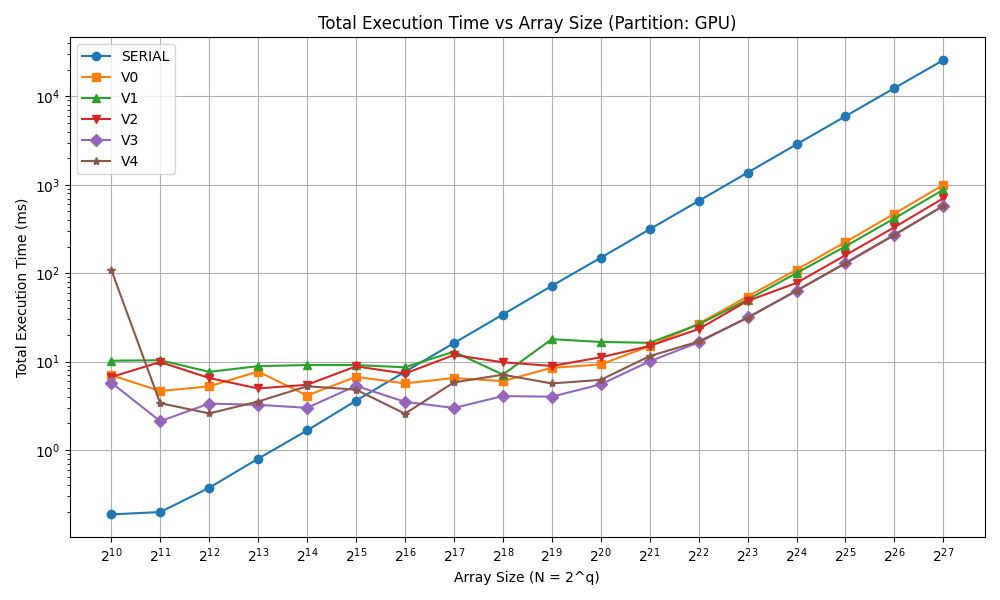
\includegraphics[width=1\linewidth]{execution_times_comparison_gpu.png}
    \caption{Total execution time for sorting arrays of increasing size using each version of Bitonic Sort on 
    the \texttt{gpu} partition (Tesla P100). The A100 shows similar trends with consistently better performance.}
    \label{fig:execution_times_comparison_gpu}
\end{figure}

\end{document}
